\subsection{Cross Section Interval Folding}
\label{sec:interval_folding}

\begin{definition}
\label{def:interval}
We consider a cross section $C$ composed of segments $ \langle s_1,s_2,\cdots,s_n \rangle$
with total length $X$ (i.e. $\sum \left| s_i\right| = X$).
If we allow this cross section to evolve for time $T$, we obtain a new cross section $C_T = \langle r_1,r_2,\cdots ,r_n \rangle$.
The evolution from $C$ to $C_T$ forms a cross section interval $\mathcal C$ of length $T$.
\end{definition}

\begin{definition}
\label{def:}
Say that the total length of the cross sections in $\mathcal C$ is $X$ (we showed in \ldots that length is conserved).
We will denote a strip of paper of size $X\times L$ as an $L$-strip.
\end{definition}

\subsubsection{Interval Folding results in Flat Strip}
\label{sec:interval_flat_strip}

In this section, we focus on a single cross section interval $\mathcal C$ with segments $\langle s_1, s_2,\cdots s_n \rangle$ evolving over time $T$.
First consider the surface traced out by an individual segment $s_i$.
Since the endpoints of $s_i$ move in a straight line, each segment traces \todo{What is a trace?} a trapezoid.

\begin{figure}[htb]
\graphicspath{{./figures/}}
    \centering
    \subfloat[] {
        \def\svgwidth{0.5\textwidth}
        \input{figures/trapezoid.pdf_tex}
        \label{fig:segment_trapezoid}
    }
    \hspace{-9em}
    \subfloat[] {
        \def\svgwidth{0.7\textwidth}
        \input{figures/trapezoid_angles.pdf_tex}
        \label{fig:trapezoid_angles}
    }
    \caption{}
    \label{fig:trapezoids}
\end{figure}

\begin{definition}
\label{def:interval_folding}
Given a cross section interval $\mathcal C$ formed from a cross section $C$ evolving over time $T$,
we define the folding of $\mathcal C$ as the surface swept out by $C$ from over time $T$.
Precisely
\begin{enumerate}
\item The folding of a the $i^{th}$ segment is the trapezoid formed by the initial and final state of the segment ($s_i$ and $r_i$).
      This forms a trapezoid of height $T$ (Figure~\ref{fig:segment_trapezoid}).
      The non-parallel sides are straight lines due to Property~\ref{pro:joint_velocity}.
      In case either the initial or final segment has length, the resulting trapezoid will be a triangle.
\item For every joint $J_i$, we attach the corresponding trapezoids for $s_i$ and $s_{i+1}$
      along the joint trajectory $\mathcal T_{J_i}$ to obtain the folding of $\mathcal C$.
\end{enumerate}
\end{definition}

First, we will show that each $\mathcal C_i$ corresponds to a $T_i$-strip.

\begin{definition}
\label{def:trapezoid}
The surface traced out by a segment $s$ is a trapezoid $Z_s$ (Figure~\ref{fig:segment_trapezoid}).
Specifically, if $L,R$ are the initial left and right endpoints of $s$, and $L',R'$ are the final endpoints,
$Z_s = LL'R'R$ is the corresponding trapezoid (Figure~\ref{fig:segment_trapezoid}).
\end{definition}

\todo[inline]{Define gluing}

\begin{lemma}
\label{lem:trapezoid_gluing_parallel}
Consider a joint $J$ with segments $l$ and $r$, which has zero orthogonal joint velocity (i.e. $\vec v_l^\shortparallel = \vec v_r^\shortparallel = 0$.
The gluing of trapezoids $Z_l$ and $Z_r$ along the joint trajectory $\mathcal T_J$ is isometric to a larger trapezoid.
This joint trajectory is actually nothing but a crease in the folded state.
\end{lemma}

\begin{figure}[!htb]
\graphicspath{{figures/trapezoidZ}}
    \centering
    %\subfloat[]{
        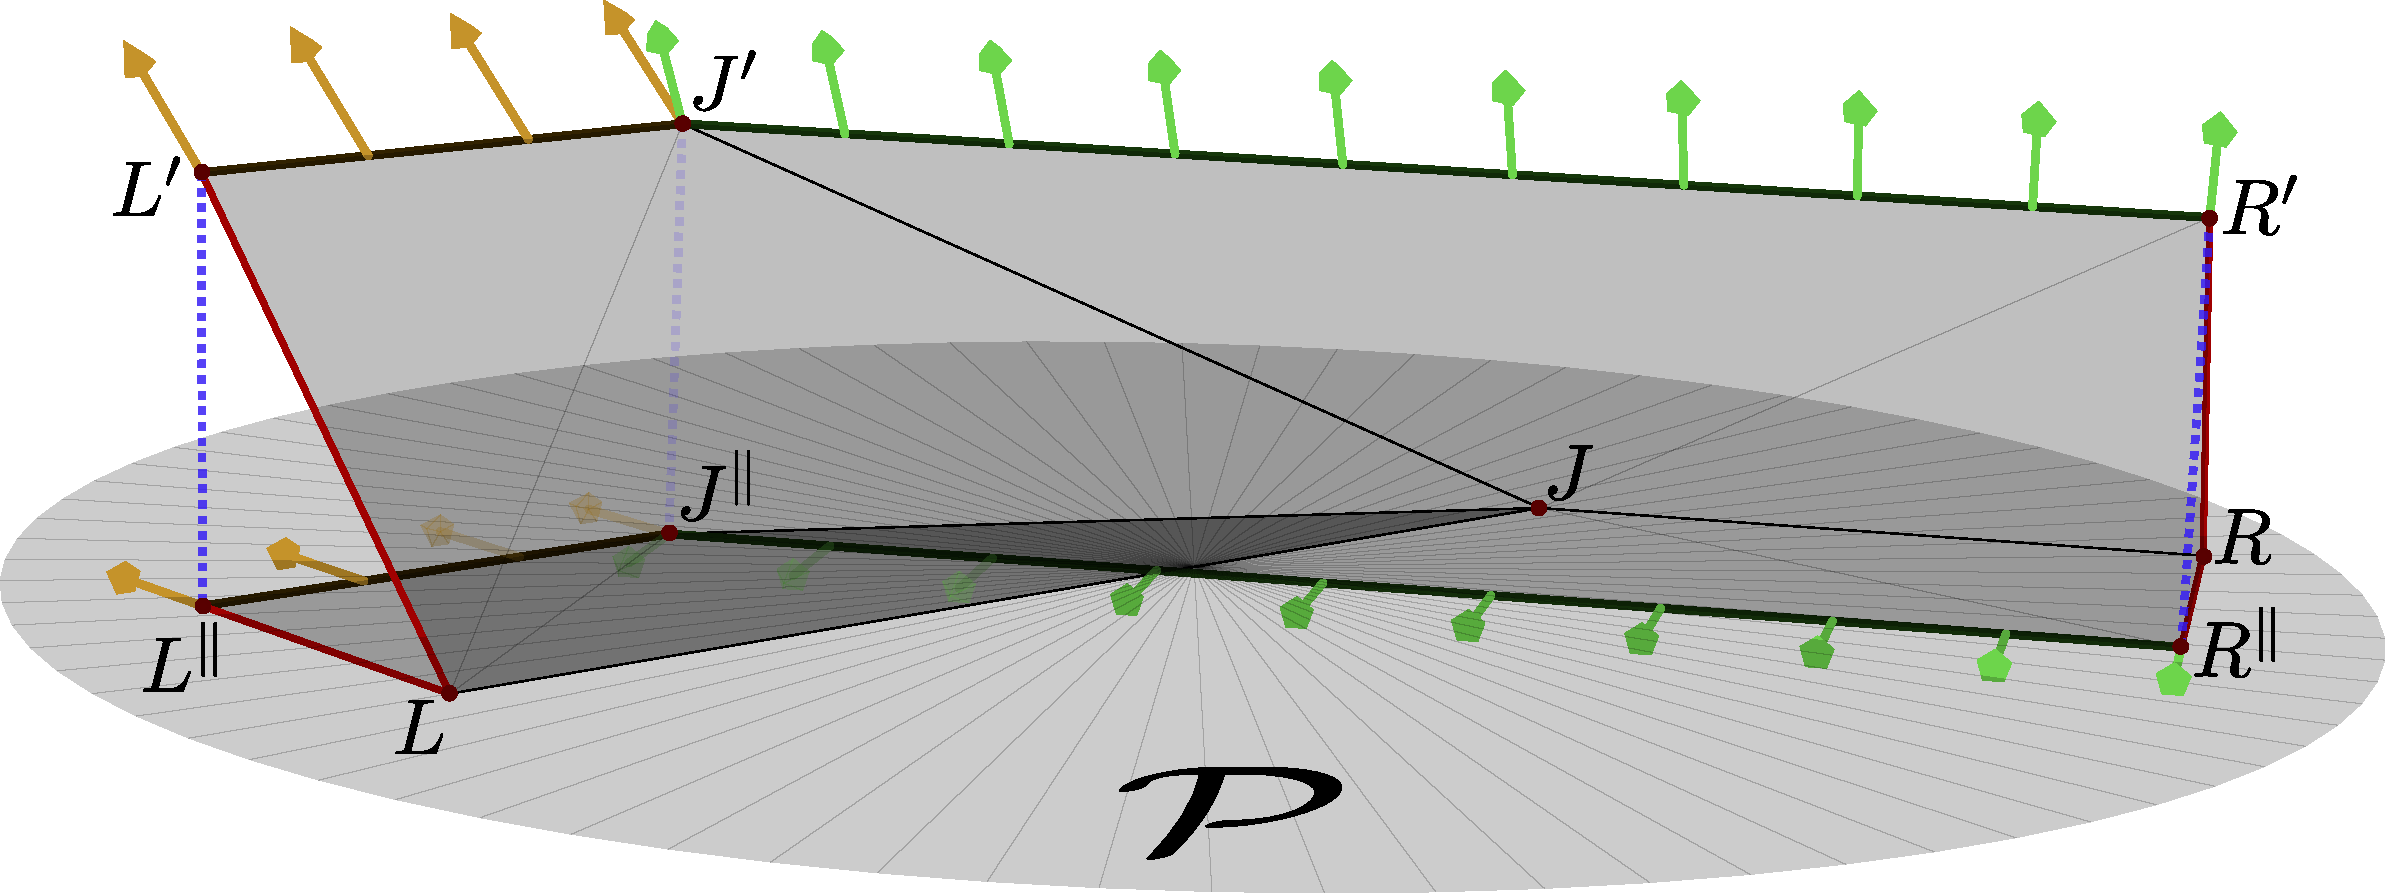
\includegraphics[width=0.5\textwidth]{figures/trapezoidZ/trapezoidZ0.pdf}%
    %}%
    %\subfloat[]{
        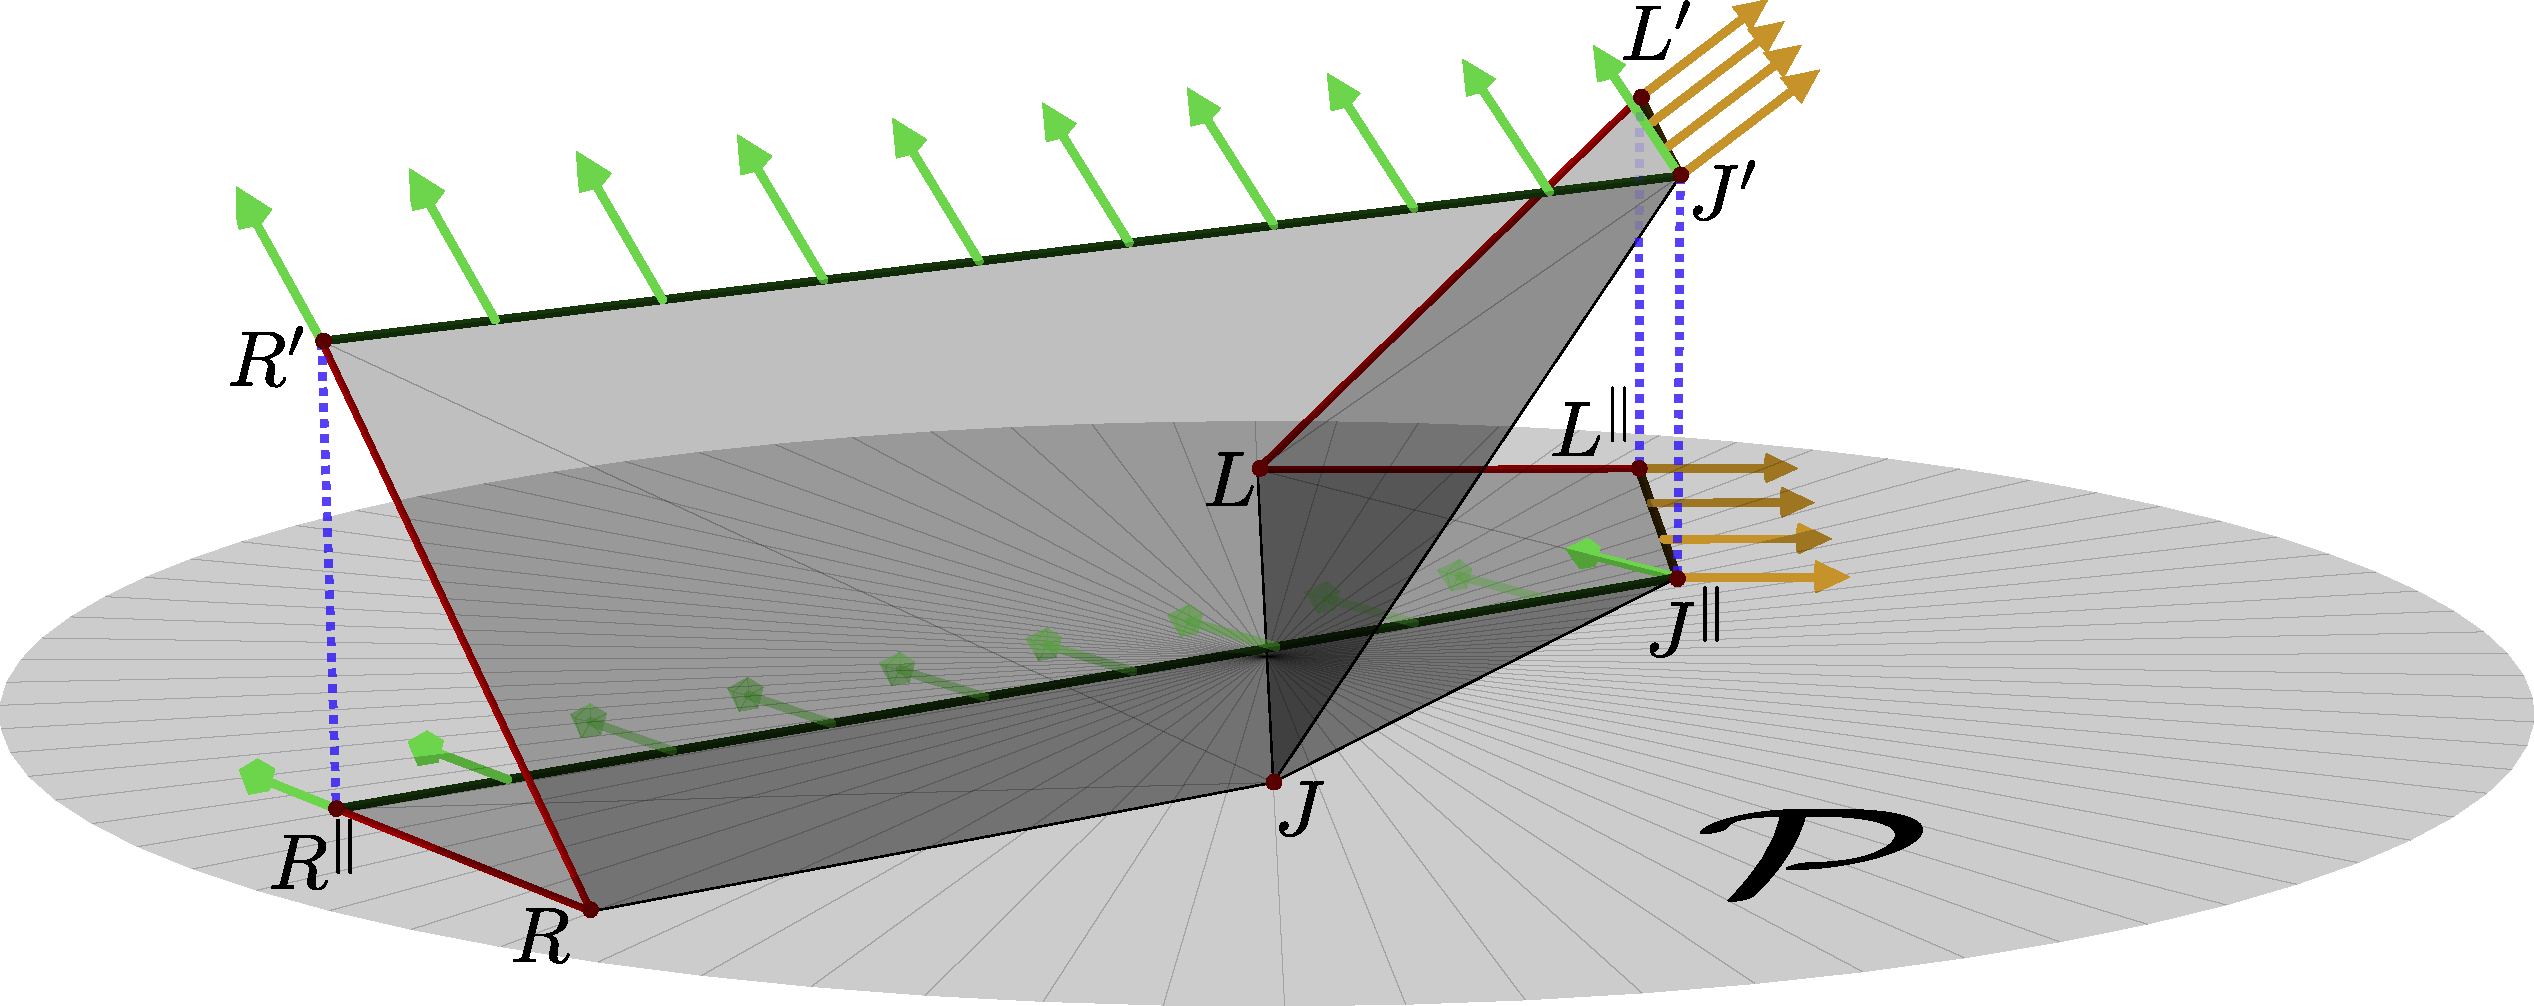
\includegraphics[width=0.5\textwidth]{figures/trapezoidZ/trapezoidZ1.pdf}%
    %}%

    %\subfloat[]{
        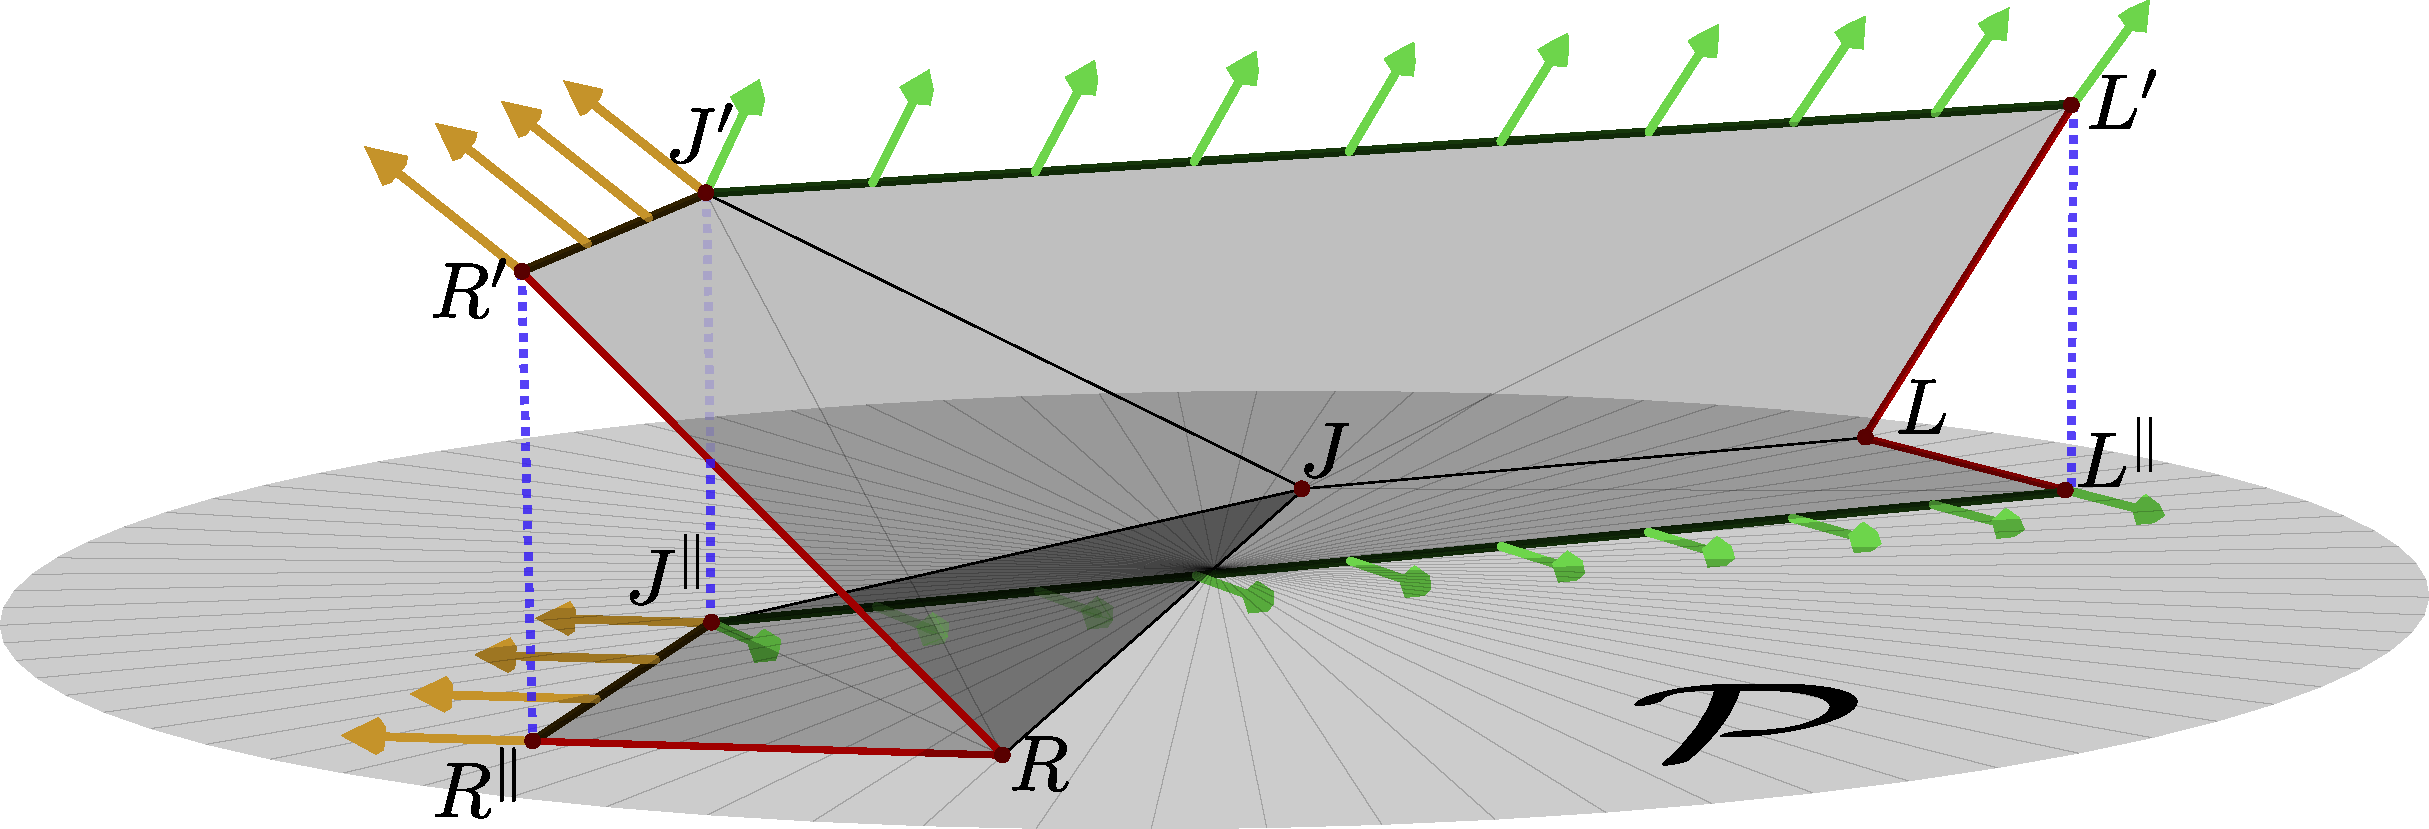
\includegraphics[width=0.8\textwidth]{figures/trapezoidZ/trapezoidZ2.pdf}%
    %}%
    \caption{
    Evolution of a joint with non-zero orthogonal velocity from $LJR$ to $L'J'R'$.
    The blue dotted lines represent the projection of the final state to the joint plane $\mathcal P$.
    }
    \label{fig:trapezoidZ}
\end{figure}

\begin{lemma}
\label{lem:trapezoid_gluing}
Consider a joint $J$ with segments $l$ and $r$ with non-zero orthogonal velocity.
The gluing of trapezoids $Z_l$ and $Z_r$ along the joint trajectory $\mathcal T_J$ is isometric to a larger trapezoid.
\end{lemma}
\begin{proof}
As before, let $LJR$ and $L'J'R'$ represent the initial and final positions of the segments respectively.
We also construct the projection of $L'J'R'$ to the joint plane $\mathcal P$ as $L^\shortparallel J^\shortparallel R^\shortparallel$.
The evolution of the projection is analogous to the setting in Lemma~\ref{lem:trapezoid_gluing_parallel}.
Therefore, $\angle LJJ^\shortparallel = \phi = \theta/2$ and $\angle RJJ^\shortparallel = \pi-\phi$.

Consider the positive $z$-axis along the joint orthogonal velocity (i.e. normal to the joint plane $\mathcal P$).
We define the orthogonal diaplacement vector as $\overrightarrow{JJ'} = z\cdot\vec{\hat k}$.
Let the positive $x$-axis be along $JJ^\shortparallel$. So, the unit vector along $\overrightarrow{JJ'}$ is $\frac{1}{\sqrt{1+z^2}}(1,0,z)$.

Since $\angle J^\shortparallel JR = \phi$, the unit vector along $\overrightarrow JR$ is $(\cos\phi,\sin\phi,0)$.
So, we compute $\cos \angle RJJ' = \cos\phi/\sqrt{1+z^2}$.
Similarly, since $\angle J^\shortparallel JL = \pi-\phi$, the unit vector along $\overrightarrow JL$ is $(-\cos\phi,\sin\phi,0)$,
which implies that $\cos \angle LJJ' = -\cos\phi/\sqrt{1+z^2}$.
Finally, since both $\angle LJJ$ and $\angle RJJ'$ are less than $\pi$, and $\cos\left(\angle LJJ' \right) = -\cos\left(\angle RJJ' \right)$,
we conclude that $\angle LJJ' + \angle RJJ' = \pi$.

Since $LJJ'L'$ and $RJJ'R'$ are both trapezoids, this implies that the resulting gluing along $JJ'$ is a larger trapezoid.
\end{proof}

\begin{theorem}
\label{thm:interval_strip}
Consider a cross section interval $\mathcal C$ formed from a cross section $C$ evolving over time $T$ to form a folding $F$.
Further assume that the total length of cross section $C$ is $X$ units. Then, $F$ is isometric to a $X\times T$ strip of paper.
\end{theorem}
\begin{proof}
From Lemma~\ref{lem:trapezoid_gluing}, we know that $F$ is isometric to a trapezoid.
Let $L,L'$ be the initial and final positions of the left (non-parallel) edge of the trapezoid, and
let $R,R'$ be the initial and final positions of the right edge of the trapezoid.
Say that $C$ comprises of segments $ \langle s_1, s_2,\cdots s_n \rangle$.
From Property~\ref{pro:left_right_velocity}, we know that the left velocity of $s_0$ is zero.
So, the line $LL'$ follows the trajectory of $\vec{\hat v_0}$, which is orthogonal to the segment $s_0$.
In other words, the left edge of the trapezoid has length $T$, and is orthogonal to the parallel edges.
Similarly, because the right velocity of $s_n$ is zero, the right edge of the trapezoid is also orthogonal.
Therefore, $F$ is isometric to a right angled trapezoid (i.e. a strip) of length $X$ and width $T$.
\end{proof}
\todo[inline]{property for NO zero length segments}

